% Options for packages loaded elsewhere
% Options for packages loaded elsewhere
\PassOptionsToPackage{unicode}{hyperref}
\PassOptionsToPackage{hyphens}{url}
\PassOptionsToPackage{dvipsnames,svgnames,x11names}{xcolor}
%
\documentclass[
  letterpaper,
  DIV=11,
  numbers=noendperiod,
  oneside]{scrartcl}
\usepackage{xcolor}
\usepackage[left=1in,marginparwidth=2.0666666666667in,textwidth=4.1333333333333in,marginparsep=0.3in]{geometry}
\usepackage{amsmath,amssymb}
\setcounter{secnumdepth}{-\maxdimen} % remove section numbering
\usepackage{iftex}
\ifPDFTeX
  \usepackage[T1]{fontenc}
  \usepackage[utf8]{inputenc}
  \usepackage{textcomp} % provide euro and other symbols
\else % if luatex or xetex
  \usepackage{unicode-math} % this also loads fontspec
  \defaultfontfeatures{Scale=MatchLowercase}
  \defaultfontfeatures[\rmfamily]{Ligatures=TeX,Scale=1}
\fi
\usepackage{lmodern}
\ifPDFTeX\else
  % xetex/luatex font selection
\fi
% Use upquote if available, for straight quotes in verbatim environments
\IfFileExists{upquote.sty}{\usepackage{upquote}}{}
\IfFileExists{microtype.sty}{% use microtype if available
  \usepackage[]{microtype}
  \UseMicrotypeSet[protrusion]{basicmath} % disable protrusion for tt fonts
}{}
\makeatletter
\@ifundefined{KOMAClassName}{% if non-KOMA class
  \IfFileExists{parskip.sty}{%
    \usepackage{parskip}
  }{% else
    \setlength{\parindent}{0pt}
    \setlength{\parskip}{6pt plus 2pt minus 1pt}}
}{% if KOMA class
  \KOMAoptions{parskip=half}}
\makeatother
% Make \paragraph and \subparagraph free-standing
\makeatletter
\ifx\paragraph\undefined\else
  \let\oldparagraph\paragraph
  \renewcommand{\paragraph}{
    \@ifstar
      \xxxParagraphStar
      \xxxParagraphNoStar
  }
  \newcommand{\xxxParagraphStar}[1]{\oldparagraph*{#1}\mbox{}}
  \newcommand{\xxxParagraphNoStar}[1]{\oldparagraph{#1}\mbox{}}
\fi
\ifx\subparagraph\undefined\else
  \let\oldsubparagraph\subparagraph
  \renewcommand{\subparagraph}{
    \@ifstar
      \xxxSubParagraphStar
      \xxxSubParagraphNoStar
  }
  \newcommand{\xxxSubParagraphStar}[1]{\oldsubparagraph*{#1}\mbox{}}
  \newcommand{\xxxSubParagraphNoStar}[1]{\oldsubparagraph{#1}\mbox{}}
\fi
\makeatother

\usepackage{color}
\usepackage{fancyvrb}
\newcommand{\VerbBar}{|}
\newcommand{\VERB}{\Verb[commandchars=\\\{\}]}
\DefineVerbatimEnvironment{Highlighting}{Verbatim}{commandchars=\\\{\}}
% Add ',fontsize=\small' for more characters per line
\newenvironment{Shaded}{}{}
\newcommand{\AlertTok}[1]{\textcolor[rgb]{1.00,0.33,0.33}{\textbf{#1}}}
\newcommand{\AnnotationTok}[1]{\textcolor[rgb]{0.42,0.45,0.49}{#1}}
\newcommand{\AttributeTok}[1]{\textcolor[rgb]{0.84,0.23,0.29}{#1}}
\newcommand{\BaseNTok}[1]{\textcolor[rgb]{0.00,0.36,0.77}{#1}}
\newcommand{\BuiltInTok}[1]{\textcolor[rgb]{0.84,0.23,0.29}{#1}}
\newcommand{\CharTok}[1]{\textcolor[rgb]{0.01,0.18,0.38}{#1}}
\newcommand{\CommentTok}[1]{\textcolor[rgb]{0.42,0.45,0.49}{#1}}
\newcommand{\CommentVarTok}[1]{\textcolor[rgb]{0.42,0.45,0.49}{#1}}
\newcommand{\ConstantTok}[1]{\textcolor[rgb]{0.00,0.36,0.77}{#1}}
\newcommand{\ControlFlowTok}[1]{\textcolor[rgb]{0.84,0.23,0.29}{#1}}
\newcommand{\DataTypeTok}[1]{\textcolor[rgb]{0.84,0.23,0.29}{#1}}
\newcommand{\DecValTok}[1]{\textcolor[rgb]{0.00,0.36,0.77}{#1}}
\newcommand{\DocumentationTok}[1]{\textcolor[rgb]{0.42,0.45,0.49}{#1}}
\newcommand{\ErrorTok}[1]{\textcolor[rgb]{1.00,0.33,0.33}{\underline{#1}}}
\newcommand{\ExtensionTok}[1]{\textcolor[rgb]{0.84,0.23,0.29}{\textbf{#1}}}
\newcommand{\FloatTok}[1]{\textcolor[rgb]{0.00,0.36,0.77}{#1}}
\newcommand{\FunctionTok}[1]{\textcolor[rgb]{0.44,0.26,0.76}{#1}}
\newcommand{\ImportTok}[1]{\textcolor[rgb]{0.01,0.18,0.38}{#1}}
\newcommand{\InformationTok}[1]{\textcolor[rgb]{0.42,0.45,0.49}{#1}}
\newcommand{\KeywordTok}[1]{\textcolor[rgb]{0.84,0.23,0.29}{#1}}
\newcommand{\NormalTok}[1]{\textcolor[rgb]{0.14,0.16,0.18}{#1}}
\newcommand{\OperatorTok}[1]{\textcolor[rgb]{0.14,0.16,0.18}{#1}}
\newcommand{\OtherTok}[1]{\textcolor[rgb]{0.44,0.26,0.76}{#1}}
\newcommand{\PreprocessorTok}[1]{\textcolor[rgb]{0.84,0.23,0.29}{#1}}
\newcommand{\RegionMarkerTok}[1]{\textcolor[rgb]{0.42,0.45,0.49}{#1}}
\newcommand{\SpecialCharTok}[1]{\textcolor[rgb]{0.00,0.36,0.77}{#1}}
\newcommand{\SpecialStringTok}[1]{\textcolor[rgb]{0.01,0.18,0.38}{#1}}
\newcommand{\StringTok}[1]{\textcolor[rgb]{0.01,0.18,0.38}{#1}}
\newcommand{\VariableTok}[1]{\textcolor[rgb]{0.89,0.38,0.04}{#1}}
\newcommand{\VerbatimStringTok}[1]{\textcolor[rgb]{0.01,0.18,0.38}{#1}}
\newcommand{\WarningTok}[1]{\textcolor[rgb]{1.00,0.33,0.33}{#1}}

\usepackage{longtable,booktabs,array}
\usepackage{calc} % for calculating minipage widths
% Correct order of tables after \paragraph or \subparagraph
\usepackage{etoolbox}
\makeatletter
\patchcmd\longtable{\par}{\if@noskipsec\mbox{}\fi\par}{}{}
\makeatother
% Allow footnotes in longtable head/foot
\IfFileExists{footnotehyper.sty}{\usepackage{footnotehyper}}{\usepackage{footnote}}
\makesavenoteenv{longtable}
\usepackage{graphicx}
\makeatletter
\newsavebox\pandoc@box
\newcommand*\pandocbounded[1]{% scales image to fit in text height/width
  \sbox\pandoc@box{#1}%
  \Gscale@div\@tempa{\textheight}{\dimexpr\ht\pandoc@box+\dp\pandoc@box\relax}%
  \Gscale@div\@tempb{\linewidth}{\wd\pandoc@box}%
  \ifdim\@tempb\p@<\@tempa\p@\let\@tempa\@tempb\fi% select the smaller of both
  \ifdim\@tempa\p@<\p@\scalebox{\@tempa}{\usebox\pandoc@box}%
  \else\usebox{\pandoc@box}%
  \fi%
}
% Set default figure placement to htbp
\def\fps@figure{htbp}
\makeatother

\ifLuaTeX
  \usepackage{luacolor}
  \usepackage[soul]{lua-ul}
\else
  \usepackage{soul}
\fi




\setlength{\emergencystretch}{3em} % prevent overfull lines

\providecommand{\tightlist}{%
  \setlength{\itemsep}{0pt}\setlength{\parskip}{0pt}}



 


\KOMAoption{captions}{tableheading}
\makeatletter
\@ifpackageloaded{tcolorbox}{}{\usepackage[skins,breakable]{tcolorbox}}
\@ifpackageloaded{fontawesome5}{}{\usepackage{fontawesome5}}
\definecolor{quarto-callout-color}{HTML}{909090}
\definecolor{quarto-callout-note-color}{HTML}{0758E5}
\definecolor{quarto-callout-important-color}{HTML}{CC1914}
\definecolor{quarto-callout-warning-color}{HTML}{EB9113}
\definecolor{quarto-callout-tip-color}{HTML}{00A047}
\definecolor{quarto-callout-caution-color}{HTML}{FC5300}
\definecolor{quarto-callout-color-frame}{HTML}{acacac}
\definecolor{quarto-callout-note-color-frame}{HTML}{4582ec}
\definecolor{quarto-callout-important-color-frame}{HTML}{d9534f}
\definecolor{quarto-callout-warning-color-frame}{HTML}{f0ad4e}
\definecolor{quarto-callout-tip-color-frame}{HTML}{02b875}
\definecolor{quarto-callout-caution-color-frame}{HTML}{fd7e14}
\makeatother
\makeatletter
\@ifpackageloaded{caption}{}{\usepackage{caption}}
\AtBeginDocument{%
\ifdefined\contentsname
  \renewcommand*\contentsname{Table of contents}
\else
  \newcommand\contentsname{Table of contents}
\fi
\ifdefined\listfigurename
  \renewcommand*\listfigurename{List of Figures}
\else
  \newcommand\listfigurename{List of Figures}
\fi
\ifdefined\listtablename
  \renewcommand*\listtablename{List of Tables}
\else
  \newcommand\listtablename{List of Tables}
\fi
\ifdefined\figurename
  \renewcommand*\figurename{Figure}
\else
  \newcommand\figurename{Figure}
\fi
\ifdefined\tablename
  \renewcommand*\tablename{Table}
\else
  \newcommand\tablename{Table}
\fi
}
\@ifpackageloaded{float}{}{\usepackage{float}}
\floatstyle{ruled}
\@ifundefined{c@chapter}{\newfloat{codelisting}{h}{lop}}{\newfloat{codelisting}{h}{lop}[chapter]}
\floatname{codelisting}{Listing}
\newcommand*\listoflistings{\listof{codelisting}{List of Listings}}
\makeatother
\makeatletter
\makeatother
\makeatletter
\@ifpackageloaded{caption}{}{\usepackage{caption}}
\@ifpackageloaded{subcaption}{}{\usepackage{subcaption}}
\makeatother
\makeatletter
\@ifpackageloaded{sidenotes}{}{\usepackage{sidenotes}}
\@ifpackageloaded{marginnote}{}{\usepackage{marginnote}}
\makeatother
\usepackage{bookmark}
\IfFileExists{xurl.sty}{\usepackage{xurl}}{} % add URL line breaks if available
\urlstyle{same}
\hypersetup{
  colorlinks=true,
  linkcolor={blue},
  filecolor={Maroon},
  citecolor={Blue},
  urlcolor={Blue},
  pdfcreator={LaTeX via pandoc}}


\author{}
\date{}
\begin{document}


\section{Module 01: Königsberg Bridge
Puzzle}\label{module-01-kuxf6nigsberg-bridge-puzzle}

Advanced Topics in Network Science

Sadamori Kojaku

skojaku@binghamton.edu

\pandocbounded{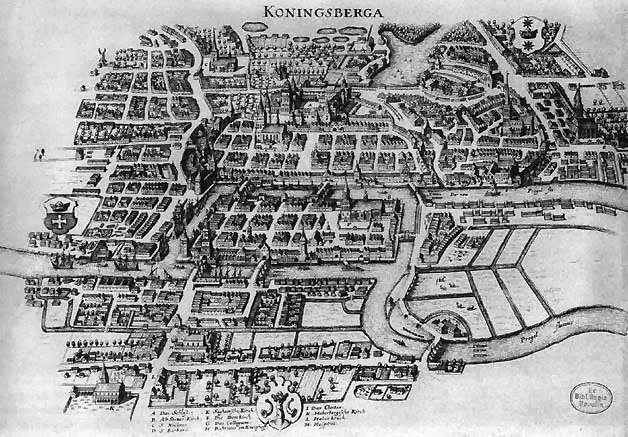
\includegraphics[keepaspectratio]{slide01_files/mediabag/Image-Koenigsberg,_M.jpg}}

\subsection{The Königsberg Bridge Puzzle
🌉}\label{the-kuxf6nigsberg-bridge-puzzle}

\begin{center}
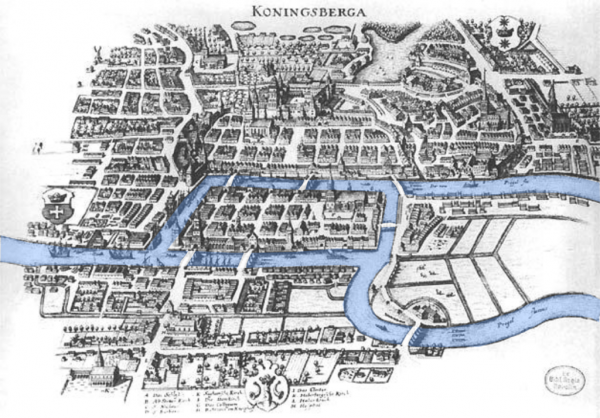
\includegraphics[width=1\linewidth,height=\textheight,keepaspectratio]{slide01_files/mediabag/bridges-with-water-6.png}
\end{center}

\begin{itemize}
\tightlist
\item
  18th century puzzle in Königsberg, Prussia (now Kaliningrad, Russia)
  🇩🇪
\item
  City had 7 bridges connecting 2 islands and mainland 🏙️
\item
  \textbf{Challenge}: Find a route that crosses each bridge exactly once
  🚶‍♂️
\end{itemize}

\subsection{Your turn! 🧩}\label{your-turn}

Find a route that crosses each bridge exactly once

Take 10 mins - Think about your strategy through the pen \& paper
exercise

\href{http://estebanmoro.org/pdf/netsci_for_kids/the_konisberg_bridges.pdf}{pen-and-paper
worksheet}

\begin{center}\rule{0.5\linewidth}{0.5pt}\end{center}

\subsubsection{Euler's Revolutionary Approach
🧠}\label{eulers-revolutionary-approach}

\textbf{What if we ignore all the physical details? 🙂 }

What do you see in this transformation? \emph{What's the key insight?}

\begin{center}
\includegraphics[width=8.33333in,height=\textheight,keepaspectratio]{slide01_files/mediabag/15n0gkvpktkGYtAase5o.png}
\end{center}

\subsection{The Breakthrough Insight ✨}\label{the-breakthrough-insight}

\textbf{Euler realized:} Only connections matter, not physical details!

\begin{itemize}
\tightlist
\item
  Landmasses → \textbf{dots} (nodes)
\item
  Bridges → \textbf{lines} (edges)
\end{itemize}

\textbf{Abstraction is the a cornerstone of Network Science}

\emph{This was the birth of graph theory and network science!}

\subsection{Euler's Reasoning 🧮}\label{eulers-reasoning}

If you walk through a node, what happens?

\begin{itemize}
\tightlist
\item
  Even number of edges: Enter/leave perfectly ✅
\item
  Odd number: One edge ``left over'' ❌
\item
  Question: Where can those ``leftover'' edges be?
\item
  Only at start/end points!
\end{itemize}

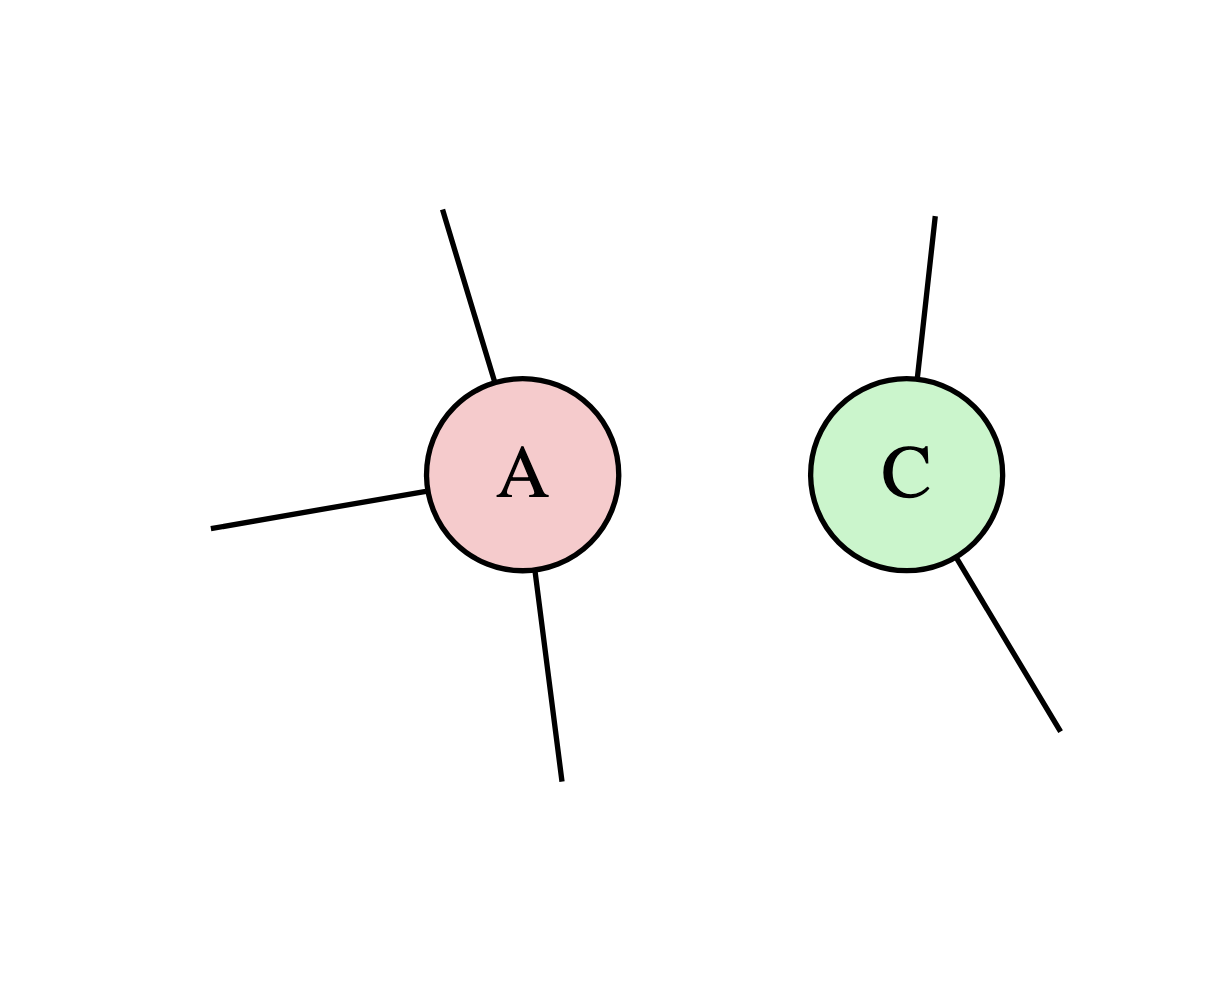
\includegraphics[width=6in,height=3in]{slide01_files/figure-latex/dot-figure-1.png}

\begin{center}\rule{0.5\linewidth}{0.5pt}\end{center}

Euler's theorem says:

\begin{itemize}
\tightlist
\item
  0 odd nodes → We can start and end at the same node while passing
  through all edges exactly once ✅
\item
  2 odd nodes → We can start and end at different nodes while passing
  through all edges exactly once ✅
\item
  More than 2 → Not possible to pass through all edges exactly once ❌
\end{itemize}

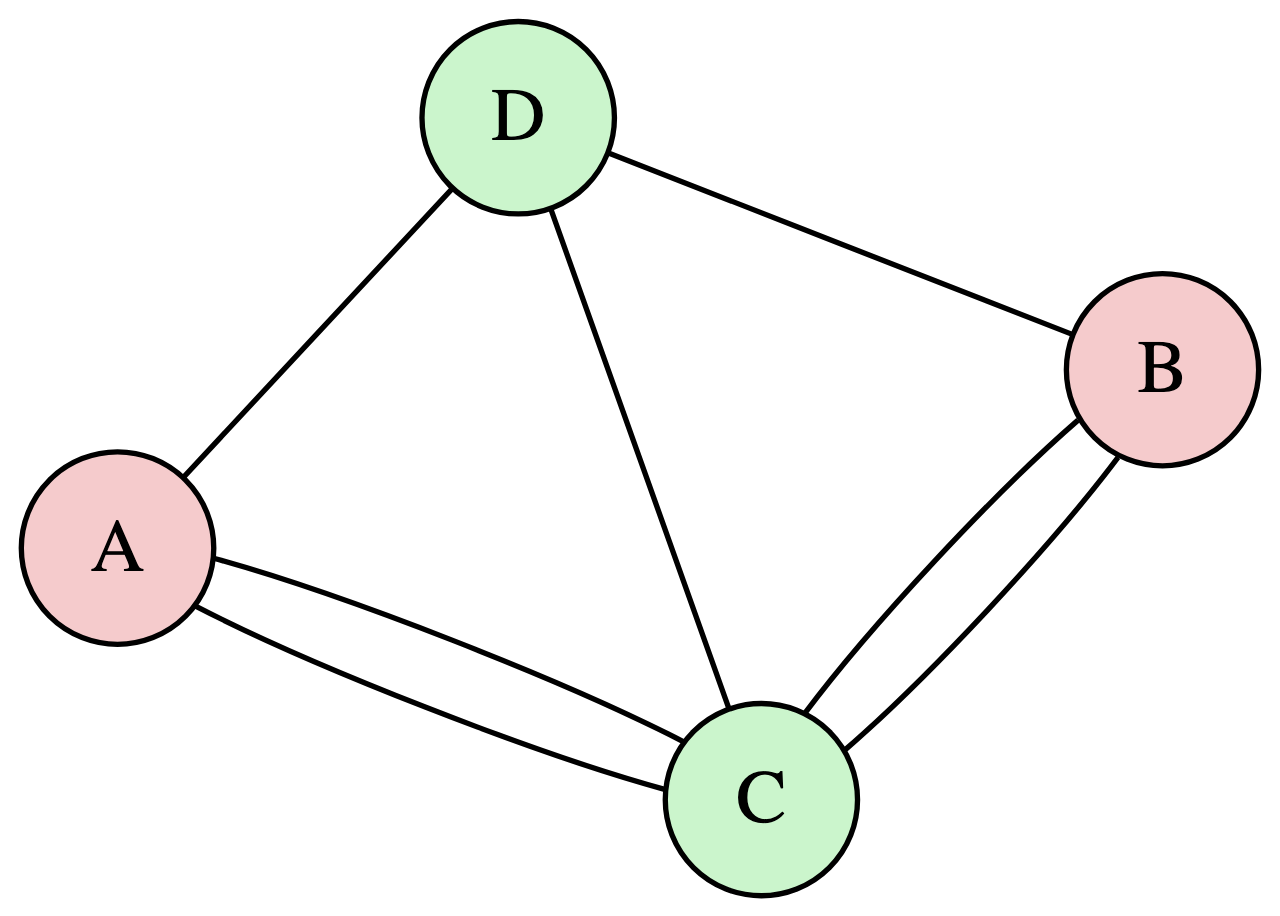
\includegraphics[width=4in,height=3in]{slide01_files/figure-latex/dot-figure-7.png}

Königsberg Bridge Problem - Seven bridges connecting four land areas

\emph{What's your verdict?}

\begin{center}\rule{0.5\linewidth}{0.5pt}\end{center}

\begin{tcolorbox}[enhanced jigsaw, opacityback=0, bottomtitle=1mm, toptitle=1mm, breakable, rightrule=.15mm, colbacktitle=quarto-callout-tip-color!10!white, toprule=.15mm, coltitle=black, colback=white, titlerule=0mm, opacitybacktitle=0.6, title=\textcolor{quarto-callout-tip-color}{\faLightbulb}\hspace{0.5em}{Euler Path Theorem}, arc=.35mm, leftrule=.75mm, bottomrule=.15mm, left=2mm, colframe=quarto-callout-tip-color-frame]

\textbf{An Euler path exists if and only if:}

\begin{enumerate}
\def\labelenumi{\arabic{enumi}.}
\tightlist
\item
  \textbf{The graph is connected} (can reach any node from any other)
\item
  \textbf{Either:}

  \begin{itemize}
  \tightlist
  \item
    All nodes have even degree (Euler circuit), OR
  \item
    Exactly two nodes have odd degree (Euler path)
  \end{itemize}
\end{enumerate}

\end{tcolorbox}

\textbf{Königsberg verdict:} 4 odd-degree nodes → \textbf{IMPOSSIBLE!}

\subsection{Aftermath}\label{aftermath}

The story takes a sobering turn during World War II. In 1944, Königsberg
was heavily bombed by Allied forces, and later captured by the Soviet
Union. Two of the seven historic bridges were destroyed in the
bombardment.

\begin{center}
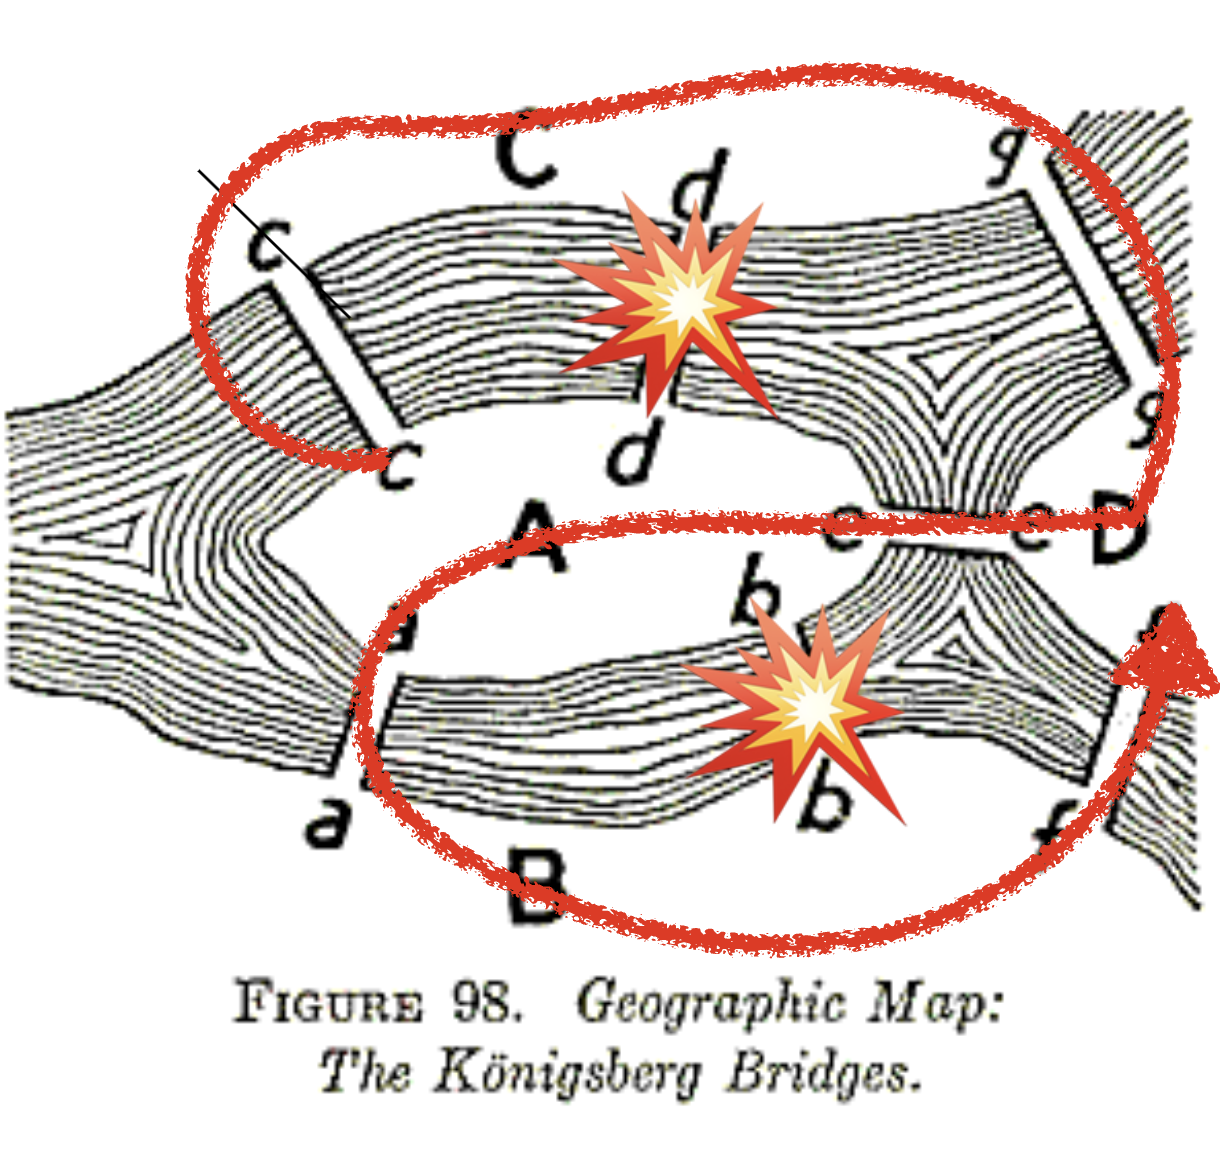
\includegraphics[width=1\linewidth,height=\textheight,keepaspectratio]{./seven-bridge-bombared.png}
\end{center}

\begin{center}\rule{0.5\linewidth}{0.5pt}\end{center}

\begin{tcolorbox}[enhanced jigsaw, opacityback=0, bottomtitle=1mm, toptitle=1mm, breakable, rightrule=.15mm, colbacktitle=quarto-callout-note-color!10!white, toprule=.15mm, coltitle=black, colback=white, titlerule=0mm, opacitybacktitle=0.6, title=\textcolor{quarto-callout-note-color}{\faInfo}\hspace{0.5em}{Question:}, arc=.35mm, leftrule=.75mm, bottomrule=.15mm, left=2mm, colframe=quarto-callout-note-color-frame]

In the previous question, we learned the condition for the possibility
to cross each bridge exactly once.

Now, let's also add a new condition: \emph{{Return to the starting
point}.}

How does this change the condition for the possibility?

\end{tcolorbox}

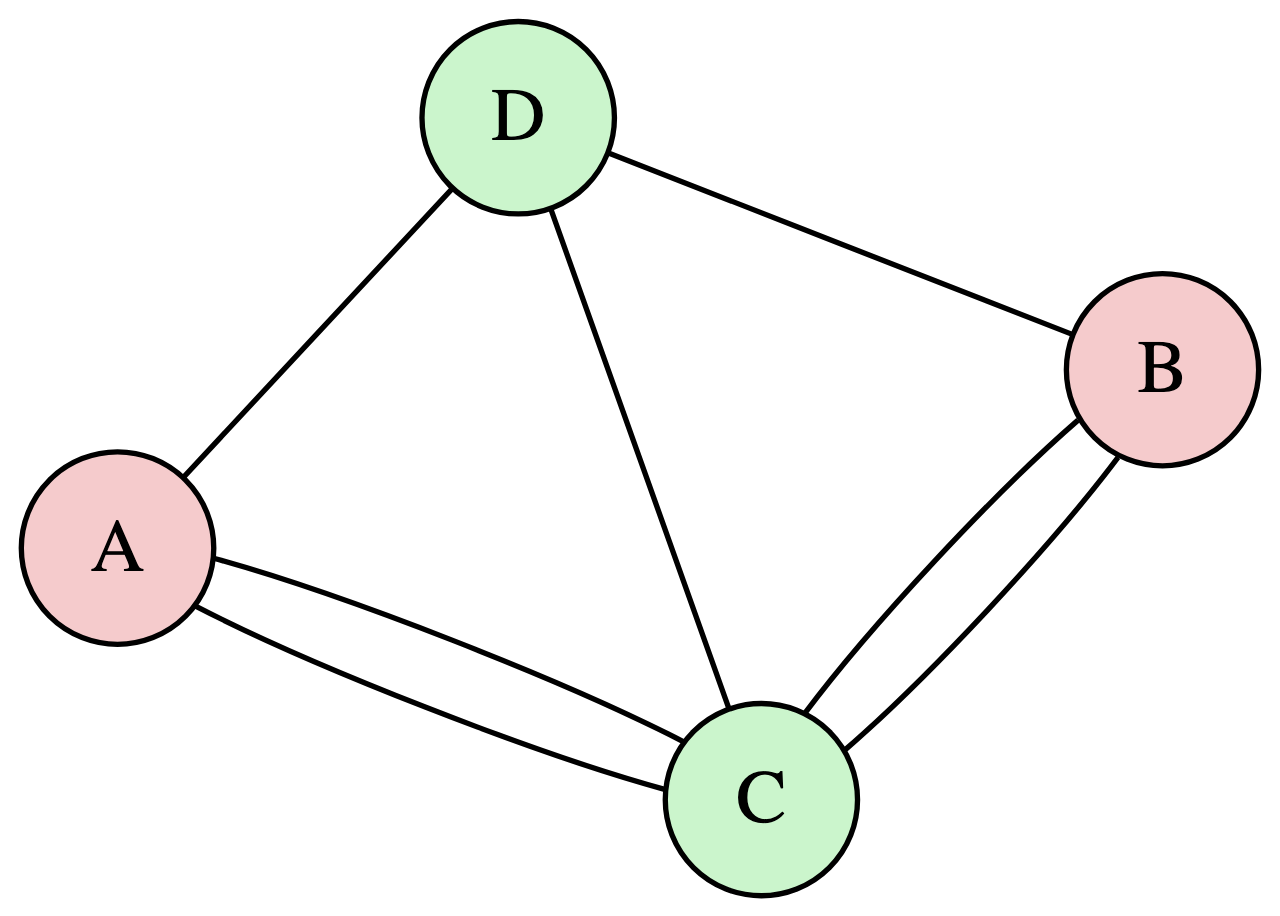
\includegraphics[width=4in,height=3in]{slide01_files/figure-latex/dot-figure-6.png}

Königsberg Bridge Problem - Seven bridges connecting four land areas

\begin{center}\rule{0.5\linewidth}{0.5pt}\end{center}

\begin{tcolorbox}[enhanced jigsaw, opacityback=0, bottomtitle=1mm, toptitle=1mm, breakable, rightrule=.15mm, colbacktitle=quarto-callout-tip-color!10!white, toprule=.15mm, coltitle=black, colback=white, titlerule=0mm, opacitybacktitle=0.6, title=\textcolor{quarto-callout-tip-color}{\faLightbulb}\hspace{0.5em}{Answer:}, arc=.35mm, leftrule=.75mm, bottomrule=.15mm, left=2mm, colframe=quarto-callout-tip-color-frame]

\begin{enumerate}
\def\labelenumi{\arabic{enumi}.}
\item
  Graph is connected, AND
\item
  Either:

  \begin{itemize}
  \tightlist
  \item
    All nodes have even degree
  \item
    \st{Exactly two nodes have odd degree}
  \end{itemize}
\end{enumerate}

This is called an {Euler circuit}.

\end{tcolorbox}

\emph{Why we cannot have odd-degree nodes?}

\begin{center}\rule{0.5\linewidth}{0.5pt}\end{center}

\begin{itemize}
\item
  \textbf{Walk}: Any sequence of connected nodes
\item
  \textbf{Path}: Walks without repeated nodes
\item
  \textbf{Circuit}: Paths that return to the starting point
\item
  \textbf{Trail}: Paths without repeated edges
\item
  \textbf{Cycle}: Trails that return to the starting point
\end{itemize}

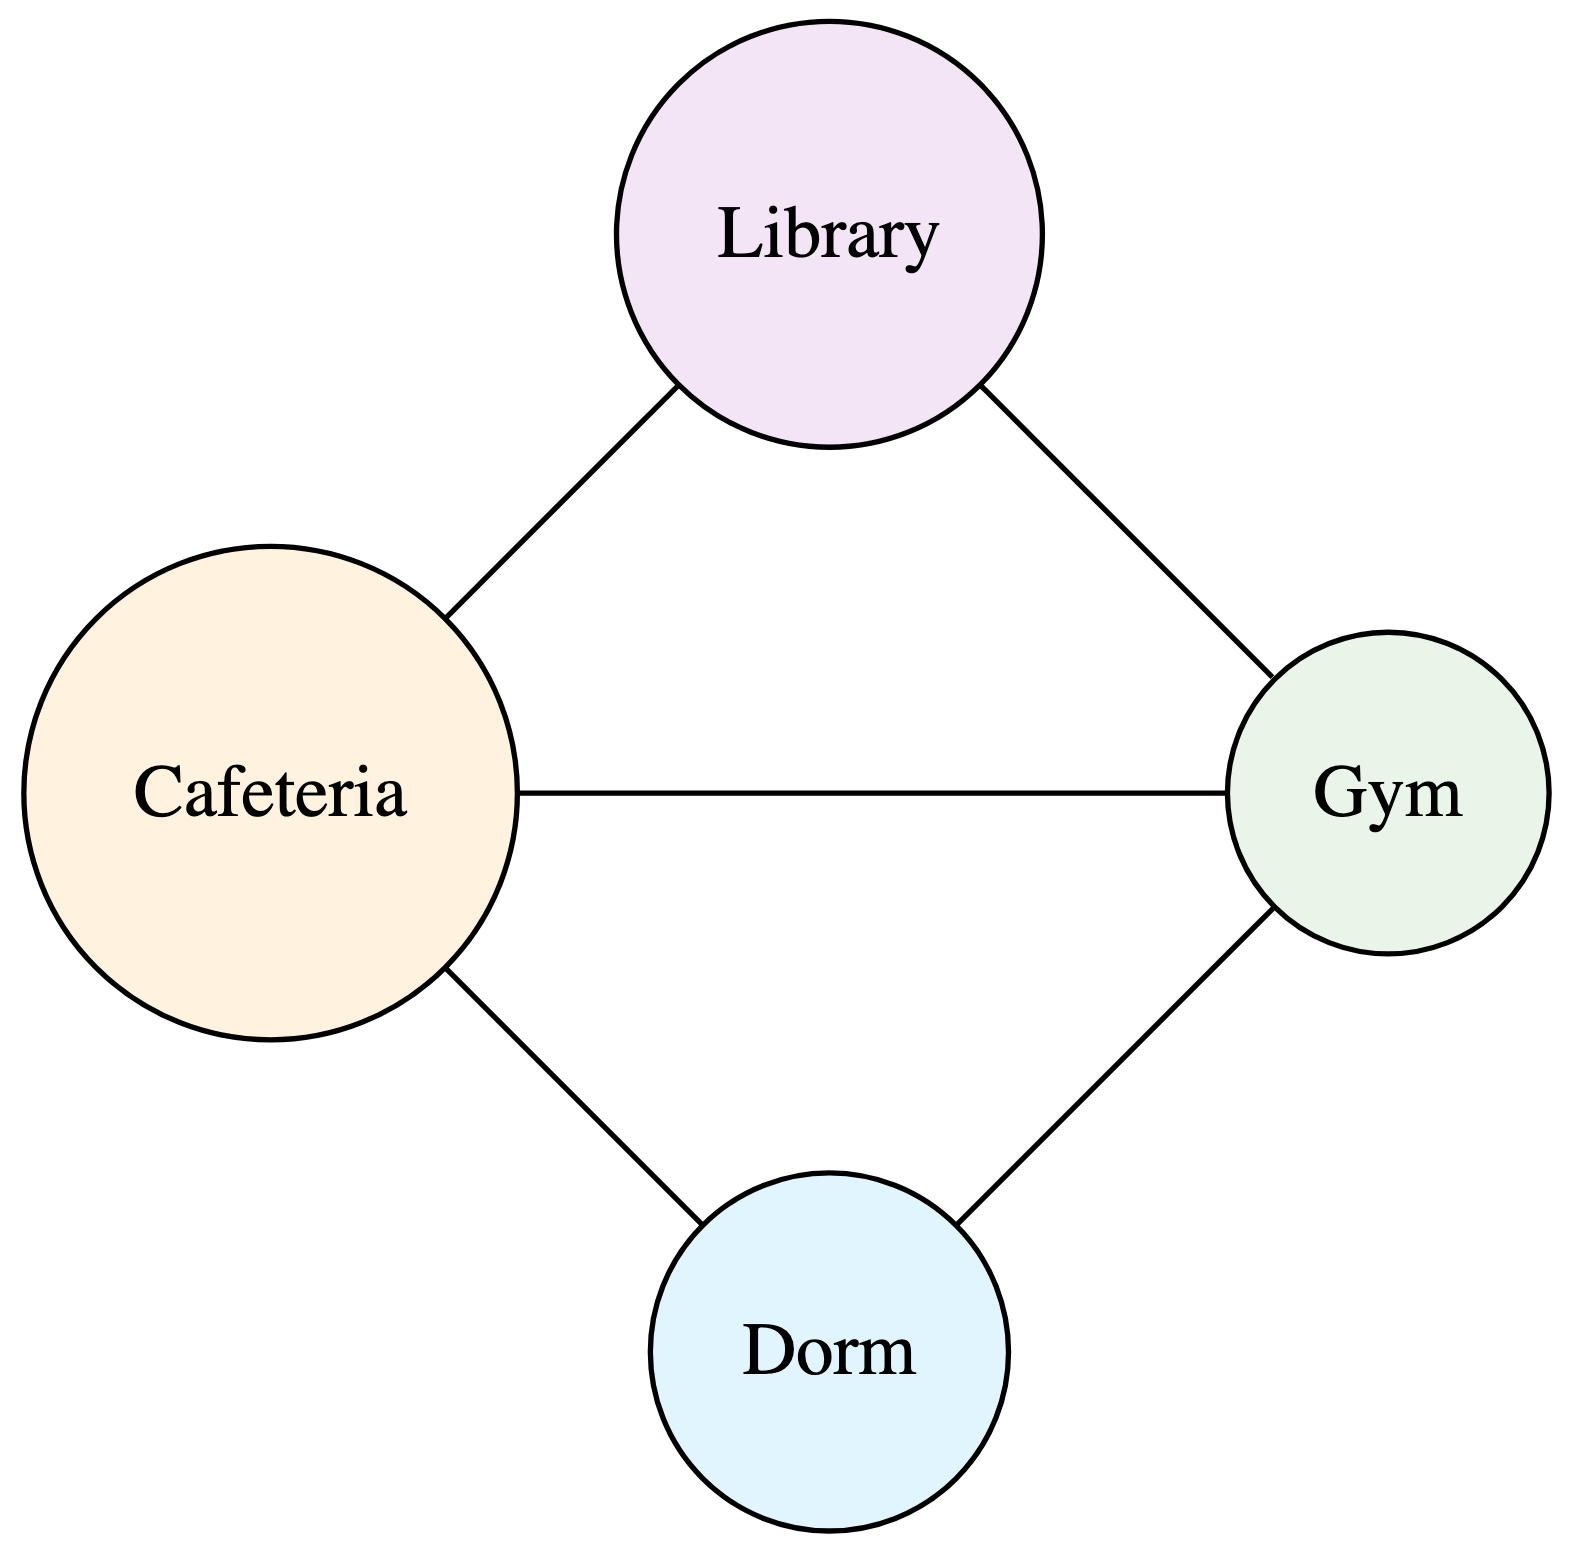
\includegraphics[width=4in,height=6in]{slide01_files/figure-latex/dot-figure-5.png}

\emph{Question: Are trails always paths? Are paths always trails?}

\subsection{Examples}\label{examples}

\begin{tcolorbox}[enhanced jigsaw, opacityback=0, bottomtitle=1mm, toptitle=1mm, breakable, rightrule=.15mm, colbacktitle=quarto-callout-note-color!10!white, toprule=.15mm, coltitle=black, colback=white, titlerule=0mm, opacitybacktitle=0.6, title=\textcolor{quarto-callout-note-color}{\faInfo}\hspace{0.5em}{Question:}, arc=.35mm, leftrule=.75mm, bottomrule=.15mm, left=2mm, colframe=quarto-callout-note-color-frame]

What are the real-world examples of the paths and trails?

\end{tcolorbox}

\begin{itemize}
\tightlist
\item
  \textbf{Path}: A travel itinerary that visits each city exactly once
\item
  \textbf{Trail}: A mail carrier's route that visits each street exactly
  once
\end{itemize}

\subsection{Network Connectivity 🔗}\label{network-connectivity}

\textbf{Look at Euler's conditions again:}

\begin{enumerate}
\def\labelenumi{\arabic{enumi}.}
\tightlist
\item
  Either all nodes have even degree OR exactly two have odd degree, and
\item
  The graph is {connected}
\end{enumerate}

What does ``connected'' mean?

\subsection{What Does ``Connected'' Really Mean?
🤔}\label{what-does-connected-really-mean}

\textbf{Definition:} {A network is \textbf{connected}} if there is a
path between every pair of nodes.

Example: You can walk from any building to any other building if
connected. A building is not connected if there is no route to it along
the walkways.

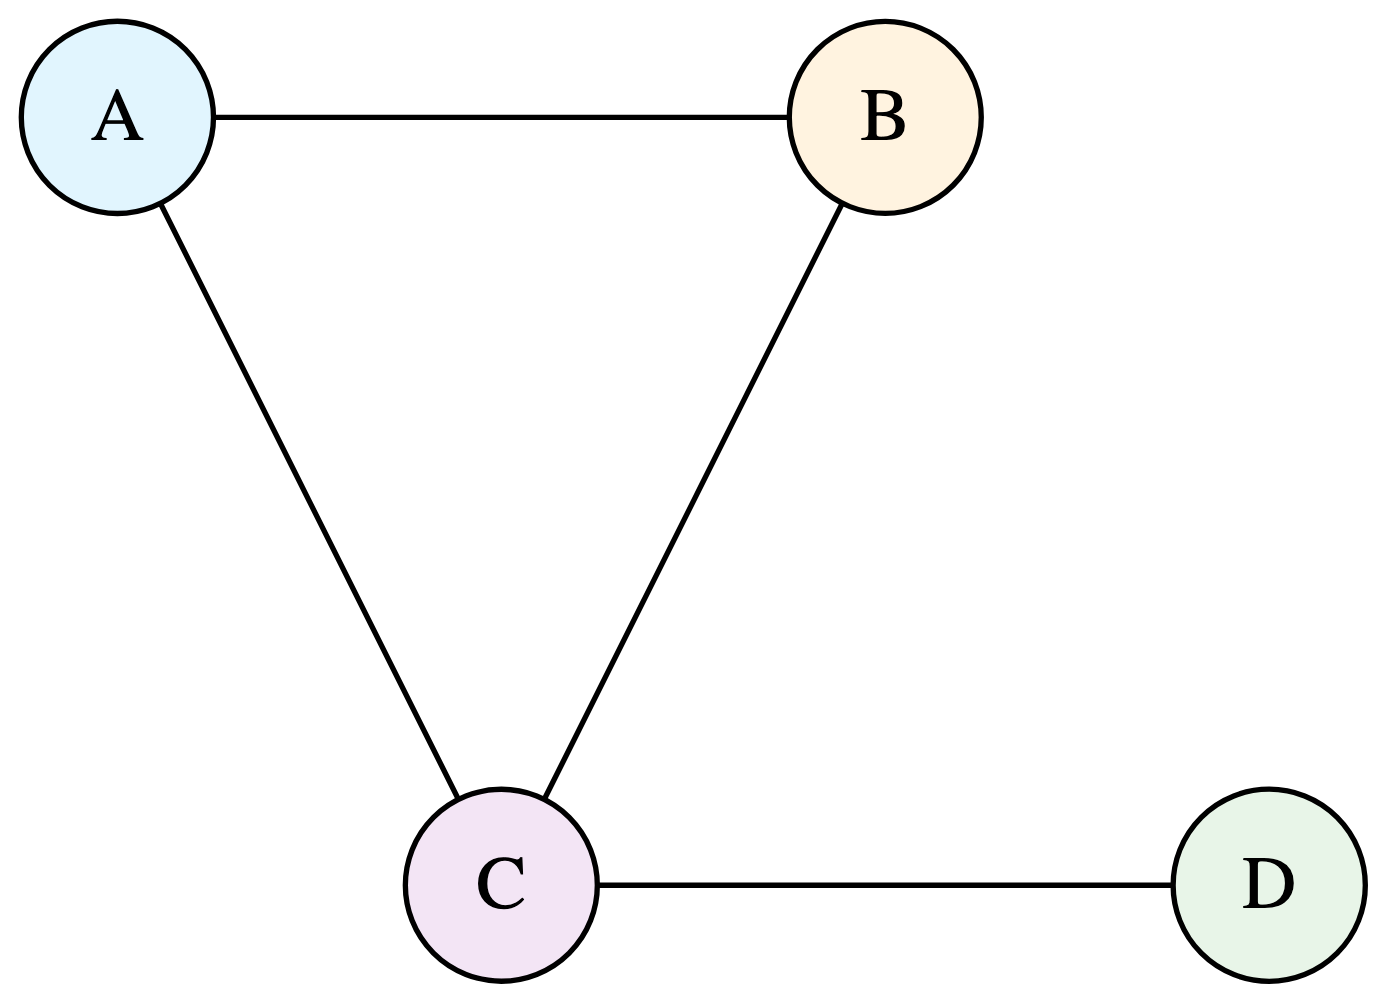
\includegraphics[width=4in,height=4in]{slide01_files/figure-latex/dot-figure-4.png}

\subsection{Connected Component}\label{connected-component}

\textbf{Definition:} {A connected component} is a maximal set of nodes
where every node can reach every other node within that set.

\begin{center}
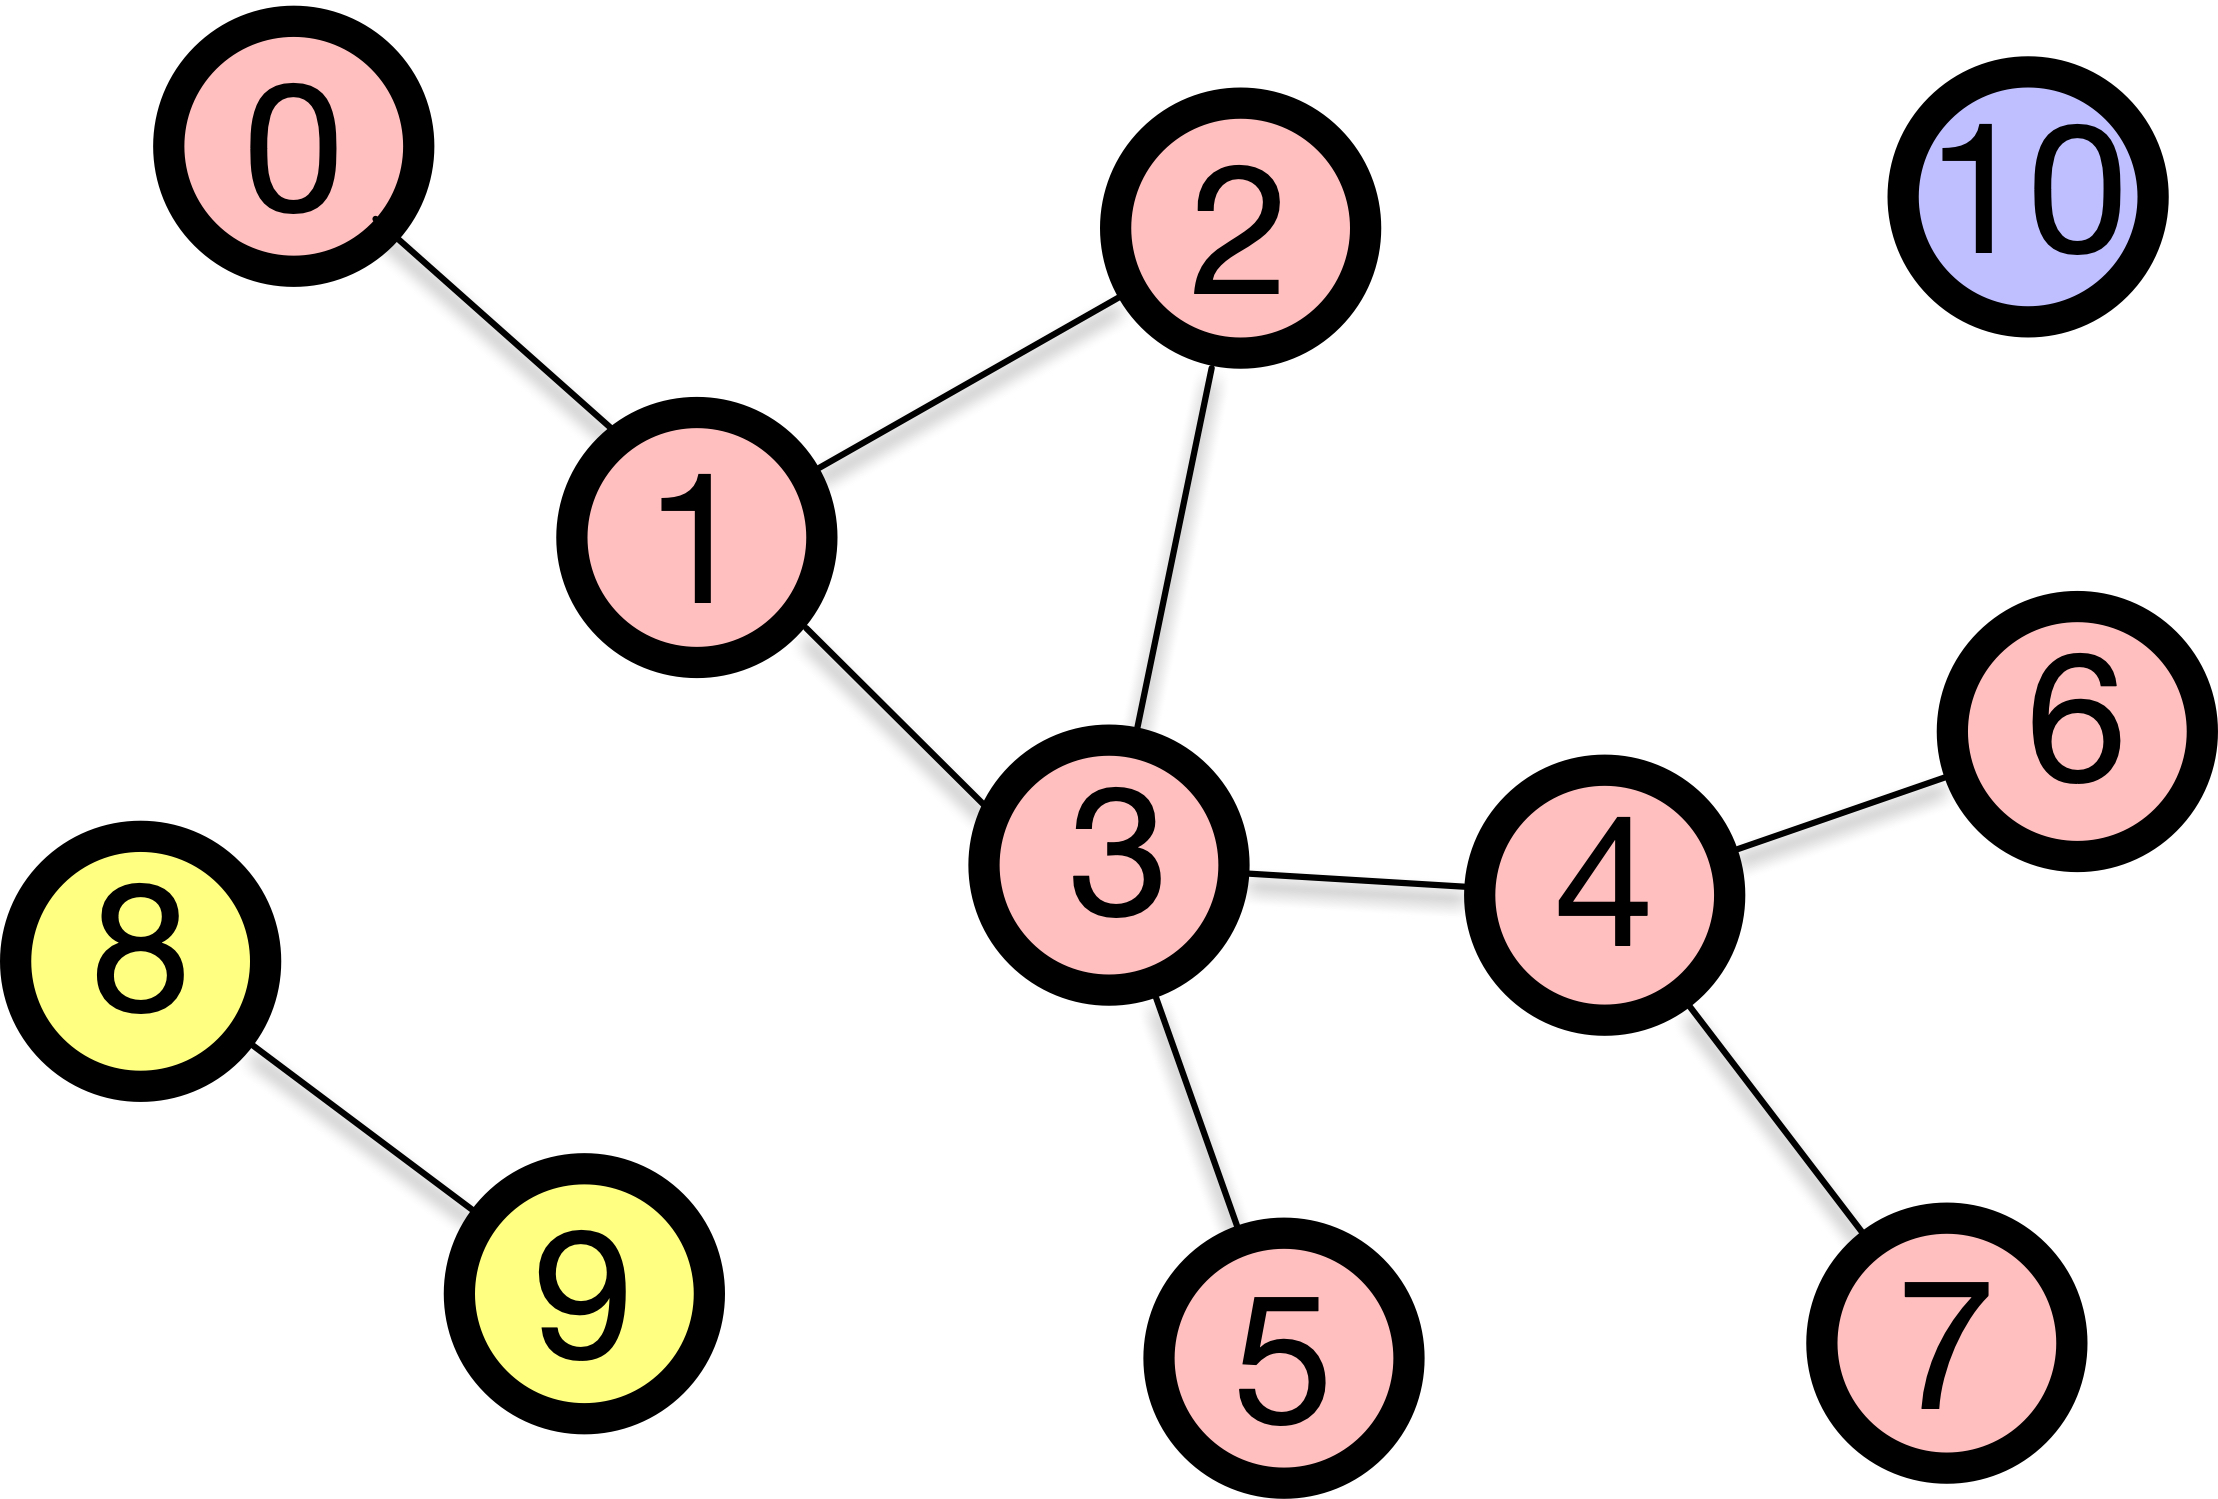
\includegraphics[width=1\linewidth,height=\textheight,keepaspectratio]{./connected-component.jpg}
\end{center}

\emph{Question: Is a single node a connected component?}

\begin{center}\rule{0.5\linewidth}{0.5pt}\end{center}

In large real-world networks, what would you expect 🤔?

\begin{itemize}
\tightlist
\item
  Many tiny components of 2-3 nodes?
\item
  One huge component containing most nodes?
\item
  All components roughly equal size?
\end{itemize}

\begin{itemize}
\tightlist
\item
  Many networks contain {a giant component} that contains a significant
  fraction of all nodes in the network
\item
  \textbf{Definition:} {A giant component} is a connected component
  where almost every node in the network is reachable from any other
  node in the component.
\end{itemize}

\begin{center}\rule{0.5\linewidth}{0.5pt}\end{center}

\textbf{Context:} What if edges have direction? (Think Twitter follows,
webpage links)

\subsubsection{Strongly connected 💪}\label{strongly-connected}

Every node can reach every other node following edge directions

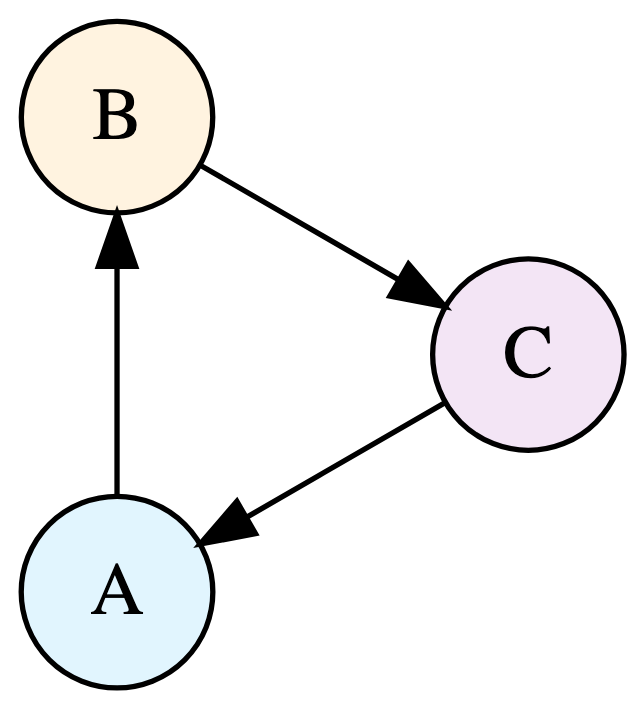
\includegraphics[width=4in,height=3in]{slide01_files/figure-latex/dot-figure-3.png}

\subsubsection{Weakly connected 🤝}\label{weakly-connected}

Connected if we ignore edge directions

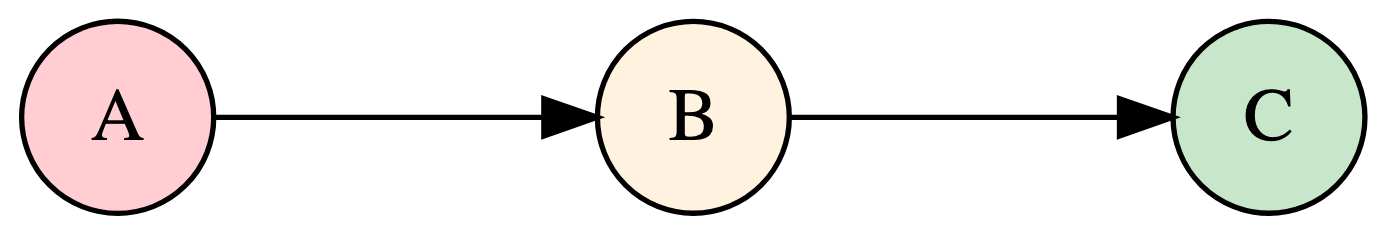
\includegraphics[width=4in,height=3in]{slide01_files/figure-latex/dot-figure-2.png}

\textbf{Question:} Is every strongly connected component also weakly
connected?

\subsection{Coding Networks in Python
💻}\label{coding-networks-in-python}

Given any network, how would you represent it in a computer?

Three ways to represent the same network:

\begin{enumerate}
\def\labelenumi{\arabic{enumi}.}
\tightlist
\item
  \textbf{Edge Table} - List of connections
\item
  \textbf{Adjacency List} - Each node's neighbors
\item
  \textbf{Adjacency Matrix} - Grid of 1s and 0s
\end{enumerate}

\begin{center}
\includegraphics[width=2.08333in,height=\textheight,keepaspectratio]{slide01_files/mediabag/tcon_a_1707286_f0001.jpg}
\end{center}

\emph{5 nodes, 6 edges}

\subsection{Edge Table: The Direct Approach
📋}\label{edge-table-the-direct-approach}

Simply list every connection:

\begin{Shaded}
\begin{Highlighting}[]
\NormalTok{edges }\OperatorTok{=}\NormalTok{ [}
\NormalTok{    (}\DecValTok{0}\NormalTok{, }\DecValTok{1}\NormalTok{),  }\CommentTok{\# Node 0 connects to Node 1}
\NormalTok{    (}\DecValTok{0}\NormalTok{, }\DecValTok{2}\NormalTok{),  }\CommentTok{\# Node 0 connects to Node 2}
\NormalTok{    (}\DecValTok{1}\NormalTok{, }\DecValTok{2}\NormalTok{),  }\CommentTok{\# Node 1 connects to Node 2}
\NormalTok{    (}\DecValTok{1}\NormalTok{, }\DecValTok{3}\NormalTok{),  }\CommentTok{\# Node 1 connects to Node 3}
\NormalTok{    (}\DecValTok{2}\NormalTok{, }\DecValTok{4}\NormalTok{),  }\CommentTok{\# Node 2 connects to Node 4}
\NormalTok{    (}\DecValTok{3}\NormalTok{, }\DecValTok{4}\NormalTok{)   }\CommentTok{\# Node 3 connects to Node 4}
\NormalTok{]}
\end{Highlighting}
\end{Shaded}

\begin{itemize}
\tightlist
\item
  \emph{How would you count the degree of node 1 from this list?}
\item
  \emph{How would you find the neighbors of node 1?}
\end{itemize}

\subsection{Adjacency List: Neighborhood Map
🗺️}\label{adjacency-list-neighborhood-map}

Each node knows its neighbors:

\begin{Shaded}
\begin{Highlighting}[]
\NormalTok{neighbors }\OperatorTok{=}\NormalTok{ \{}
    \DecValTok{0}\NormalTok{: [}\DecValTok{1}\NormalTok{, }\DecValTok{2}\NormalTok{],     }\CommentTok{\# Node 0 connects to nodes 1,2}
    \DecValTok{1}\NormalTok{: [}\DecValTok{0}\NormalTok{, }\DecValTok{2}\NormalTok{, }\DecValTok{3}\NormalTok{],  }\CommentTok{\# Node 1 connects to nodes 0,2,3}
    \DecValTok{2}\NormalTok{: [}\DecValTok{0}\NormalTok{, }\DecValTok{1}\NormalTok{, }\DecValTok{4}\NormalTok{],  }\CommentTok{\# Node 2 connects to nodes 0,1,4}
    \DecValTok{3}\NormalTok{: [}\DecValTok{1}\NormalTok{, }\DecValTok{4}\NormalTok{],     }\CommentTok{\# Node 3 connects to nodes 1,4}
    \DecValTok{4}\NormalTok{: [}\DecValTok{2}\NormalTok{, }\DecValTok{3}\NormalTok{]      }\CommentTok{\# Node 4 connects to nodes 2,3}
\NormalTok{\}}
\end{Highlighting}
\end{Shaded}

\begin{itemize}
\tightlist
\item
  \emph{How would you count the degree of node 1 from this list?}
\item
  \emph{How would you find the neighbors of node 1?}
\end{itemize}

\subsection{Adjacency Matrix: The Math Way
📐}\label{adjacency-matrix-the-math-way}

Grid where entry \((i,j) = 1\) if connected:

\begin{Shaded}
\begin{Highlighting}[]
\ImportTok{import}\NormalTok{ numpy }\ImportTok{as}\NormalTok{ np}

\NormalTok{matrix }\OperatorTok{=}\NormalTok{ np.array([}
\NormalTok{    [}\DecValTok{0}\NormalTok{, }\DecValTok{1}\NormalTok{, }\DecValTok{1}\NormalTok{, }\DecValTok{0}\NormalTok{, }\DecValTok{0}\NormalTok{],  }\CommentTok{\# Node 0: connects to 1,2}
\NormalTok{    [}\DecValTok{1}\NormalTok{, }\DecValTok{0}\NormalTok{, }\DecValTok{1}\NormalTok{, }\DecValTok{1}\NormalTok{, }\DecValTok{0}\NormalTok{],  }\CommentTok{\# Node 1: connects to 0,2,3}
\NormalTok{    [}\DecValTok{1}\NormalTok{, }\DecValTok{1}\NormalTok{, }\DecValTok{0}\NormalTok{, }\DecValTok{0}\NormalTok{, }\DecValTok{1}\NormalTok{],  }\CommentTok{\# Node 2: connects to 0,1,4}
\NormalTok{    [}\DecValTok{0}\NormalTok{, }\DecValTok{1}\NormalTok{, }\DecValTok{0}\NormalTok{, }\DecValTok{0}\NormalTok{, }\DecValTok{1}\NormalTok{],  }\CommentTok{\# Node 3: connects to 1,4}
\NormalTok{    [}\DecValTok{0}\NormalTok{, }\DecValTok{0}\NormalTok{, }\DecValTok{1}\NormalTok{, }\DecValTok{1}\NormalTok{, }\DecValTok{0}\NormalTok{]   }\CommentTok{\# Node 4: connects to 2,3}
\NormalTok{])}
\end{Highlighting}
\end{Shaded}

\begin{itemize}
\tightlist
\item
  \emph{How would you count the degree of node 1 from this matrix?}
\item
  \emph{How would you find the neighbors of node 1?}
\end{itemize}

\subsection{Implementing Euler's Theorem
🧮}\label{implementing-eulers-theorem}

\begin{Shaded}
\begin{Highlighting}[]
\KeywordTok{def}\NormalTok{ has\_euler\_path(adjacency\_matrix):}
    \CommentTok{\# Calculate degrees}
\NormalTok{    degrees }\OperatorTok{=}\NormalTok{ adjacency\_matrix.}\BuiltInTok{sum}\NormalTok{(axis}\OperatorTok{=}\DecValTok{1}\NormalTok{)}

    \CommentTok{\# Count odd degrees}
\NormalTok{    odd\_count }\OperatorTok{=} \BuiltInTok{sum}\NormalTok{(}\DecValTok{1} \ControlFlowTok{for}\NormalTok{ d }\KeywordTok{in}\NormalTok{ degrees }\ControlFlowTok{if}\NormalTok{ d }\OperatorTok{\%} \DecValTok{2} \OperatorTok{==} \DecValTok{1}\NormalTok{)}

    \CommentTok{\# Euler\textquotesingle{}s condition}
    \ControlFlowTok{return}\NormalTok{ odd\_count }\OperatorTok{==} \DecValTok{0} \KeywordTok{or}\NormalTok{ odd\_count }\OperatorTok{==} \DecValTok{2}
\end{Highlighting}
\end{Shaded}

\emph{Do you agree with this?}

\subsection{The Missing Piece: Connectivity
⚖️}\label{the-missing-piece-connectivity}

\begin{tcolorbox}[enhanced jigsaw, opacityback=0, bottomtitle=1mm, toptitle=1mm, breakable, rightrule=.15mm, colbacktitle=quarto-callout-tip-color!10!white, toprule=.15mm, coltitle=black, colback=white, titlerule=0mm, opacitybacktitle=0.6, title=\textcolor{quarto-callout-tip-color}{\faLightbulb}\hspace{0.5em}{Revisit}, arc=.35mm, leftrule=.75mm, bottomrule=.15mm, left=2mm, colframe=quarto-callout-tip-color-frame]

An Euler path exists if and only if:

\begin{enumerate}
\def\labelenumi{\arabic{enumi}.}
\tightlist
\item
  \textbf{The graph is connected} ← We forgot this!
\item
  \textbf{Exactly 0 or 2 nodes have odd degree}
\end{enumerate}

\end{tcolorbox}

\section{Module 01 Review 🎯}\label{module-01-review}

\begin{center}\rule{0.5\linewidth}{0.5pt}\end{center}

\begin{itemize}
\tightlist
\item
  \textbf{Euler's legacy} (1736)

  \begin{itemize}
  \tightlist
  \item
    Abstraction over physical details
  \item
    Focus on relationships \(\rightarrow\) Birth of graph theory
  \end{itemize}
\item
  \textbf{Euler's theorem}

  \begin{itemize}
  \tightlist
  \item
    {Euler path} exists if and only if the graph is {connected} and
    exactly 0 or 2 nodes have odd {degree}
  \end{itemize}
\item
  \textbf{Key concepts}:

  \begin{itemize}
  \tightlist
  \item
    Path, walk, trail, circuit, cycle
  \item
    Connected component, giant component, degree
  \end{itemize}
\item
  \textbf{Computational Representation}

  \begin{itemize}
  \tightlist
  \item
    Edge table, adjacency list, adjacency matrix
  \end{itemize}
\end{itemize}

\begin{center}\rule{0.5\linewidth}{0.5pt}\end{center}

\begin{itemize}
\tightlist
\item
  \textbf{Walk}

  \begin{itemize}
  \tightlist
  \item
    Any sequence of connected nodes
  \end{itemize}
\item
  \textbf{Trail}

  \begin{itemize}
  \tightlist
  \item
    Walk without repeated edges
  \end{itemize}
\item
  \textbf{Path}

  \begin{itemize}
  \tightlist
  \item
    Walk without repeated nodes
  \end{itemize}
\item
  \textbf{Circuit/Cycle:}

  \begin{itemize}
  \tightlist
  \item
    Closed versions that return to start
  \end{itemize}
\item
  {Is a path always a trail 🤔?}

  \begin{itemize}
  \tightlist
  \item
    {Yes. Path does not repeat edges.}
  \end{itemize}
\end{itemize}

\begin{center}\rule{0.5\linewidth}{0.5pt}\end{center}

\begin{itemize}
\tightlist
\item
  \textbf{Connected}

  \begin{itemize}
  \tightlist
  \item
    A network where there is a path between every pair of nodes
  \end{itemize}
\item
  \textbf{Connected component}

  \begin{itemize}
  \tightlist
  \item
    A maximal set of nodes where every node can reach every other node
    within that set
  \end{itemize}
\item
  \textbf{Giant component}

  \begin{itemize}
  \tightlist
  \item
    A connected component where almost every node in the network is
    reachable from any other node in the component
  \end{itemize}
\item
  \textbf{Strongly connected}

  \begin{itemize}
  \tightlist
  \item
    A network where every node can reach every other node following edge
    directions
  \end{itemize}
\item
  \textbf{Weakly connected}

  \begin{itemize}
  \tightlist
  \item
    A network where there is a path between every pair of nodes ignoring
    edge directions
  \end{itemize}
\end{itemize}

\begin{center}\rule{0.5\linewidth}{0.5pt}\end{center}

\begin{itemize}
\tightlist
\item
  \textbf{Euler path}

  \begin{itemize}
  \tightlist
  \item
    A path that visits each edge exactly once
  \end{itemize}
\item
  \textbf{Euler circuit}

  \begin{itemize}
  \tightlist
  \item
    An Euler path that starts and ends at the same node
  \end{itemize}
\item
  {What is the condition for the existence of an Euler circuit?}

  \begin{itemize}
  \tightlist
  \item
    {Graph is connected and all nodes have even degree.}
  \end{itemize}
\end{itemize}

\begin{center}\rule{0.5\linewidth}{0.5pt}\end{center}

\subsection{Representation of
Networks}\label{representation-of-networks}

\textbf{Edge Table}

\begin{Shaded}
\begin{Highlighting}[]
\NormalTok{edges }\OperatorTok{=}\NormalTok{ [}
\NormalTok{    (}\DecValTok{0}\NormalTok{, }\DecValTok{1}\NormalTok{),}
\NormalTok{    (}\DecValTok{1}\NormalTok{, }\DecValTok{2}\NormalTok{),}
\NormalTok{    (}\DecValTok{2}\NormalTok{, }\DecValTok{3}\NormalTok{)}
\NormalTok{]}
\end{Highlighting}
\end{Shaded}

\emph{Best for:} Storage, I/O

\textbf{Adjacency List}

\begin{Shaded}
\begin{Highlighting}[]
\NormalTok{neighbors }\OperatorTok{=}\NormalTok{ \{}
    \DecValTok{0}\NormalTok{: [}\DecValTok{1}\NormalTok{],}
    \DecValTok{1}\NormalTok{: [}\DecValTok{0}\NormalTok{, }\DecValTok{2}\NormalTok{],}
    \DecValTok{2}\NormalTok{: [}\DecValTok{1}\NormalTok{, }\DecValTok{3}\NormalTok{]}
\NormalTok{\}}
\end{Highlighting}
\end{Shaded}

\emph{Best for:} Neighbor search

\textbf{Adjacency Matrix}

\begin{Shaded}
\begin{Highlighting}[]
\NormalTok{matrix }\OperatorTok{=}\NormalTok{ np.array([}
\NormalTok{    [}\DecValTok{0}\NormalTok{, }\DecValTok{1}\NormalTok{, }\DecValTok{0}\NormalTok{],}
\NormalTok{    [}\DecValTok{1}\NormalTok{, }\DecValTok{0}\NormalTok{, }\DecValTok{1}\NormalTok{],}
\NormalTok{    [}\DecValTok{0}\NormalTok{, }\DecValTok{1}\NormalTok{, }\DecValTok{0}\NormalTok{]}
\NormalTok{])}
\end{Highlighting}
\end{Shaded}

\emph{Best for:} Math operations

\textbf{My recommendation:}

Use edge table for saving the network data. Use (sparse) adjacency
matrices for analysis.

\subsection{Coming up in Module 02:}\label{coming-up-in-module-02}

\textbf{Small world networks}

\pandocbounded{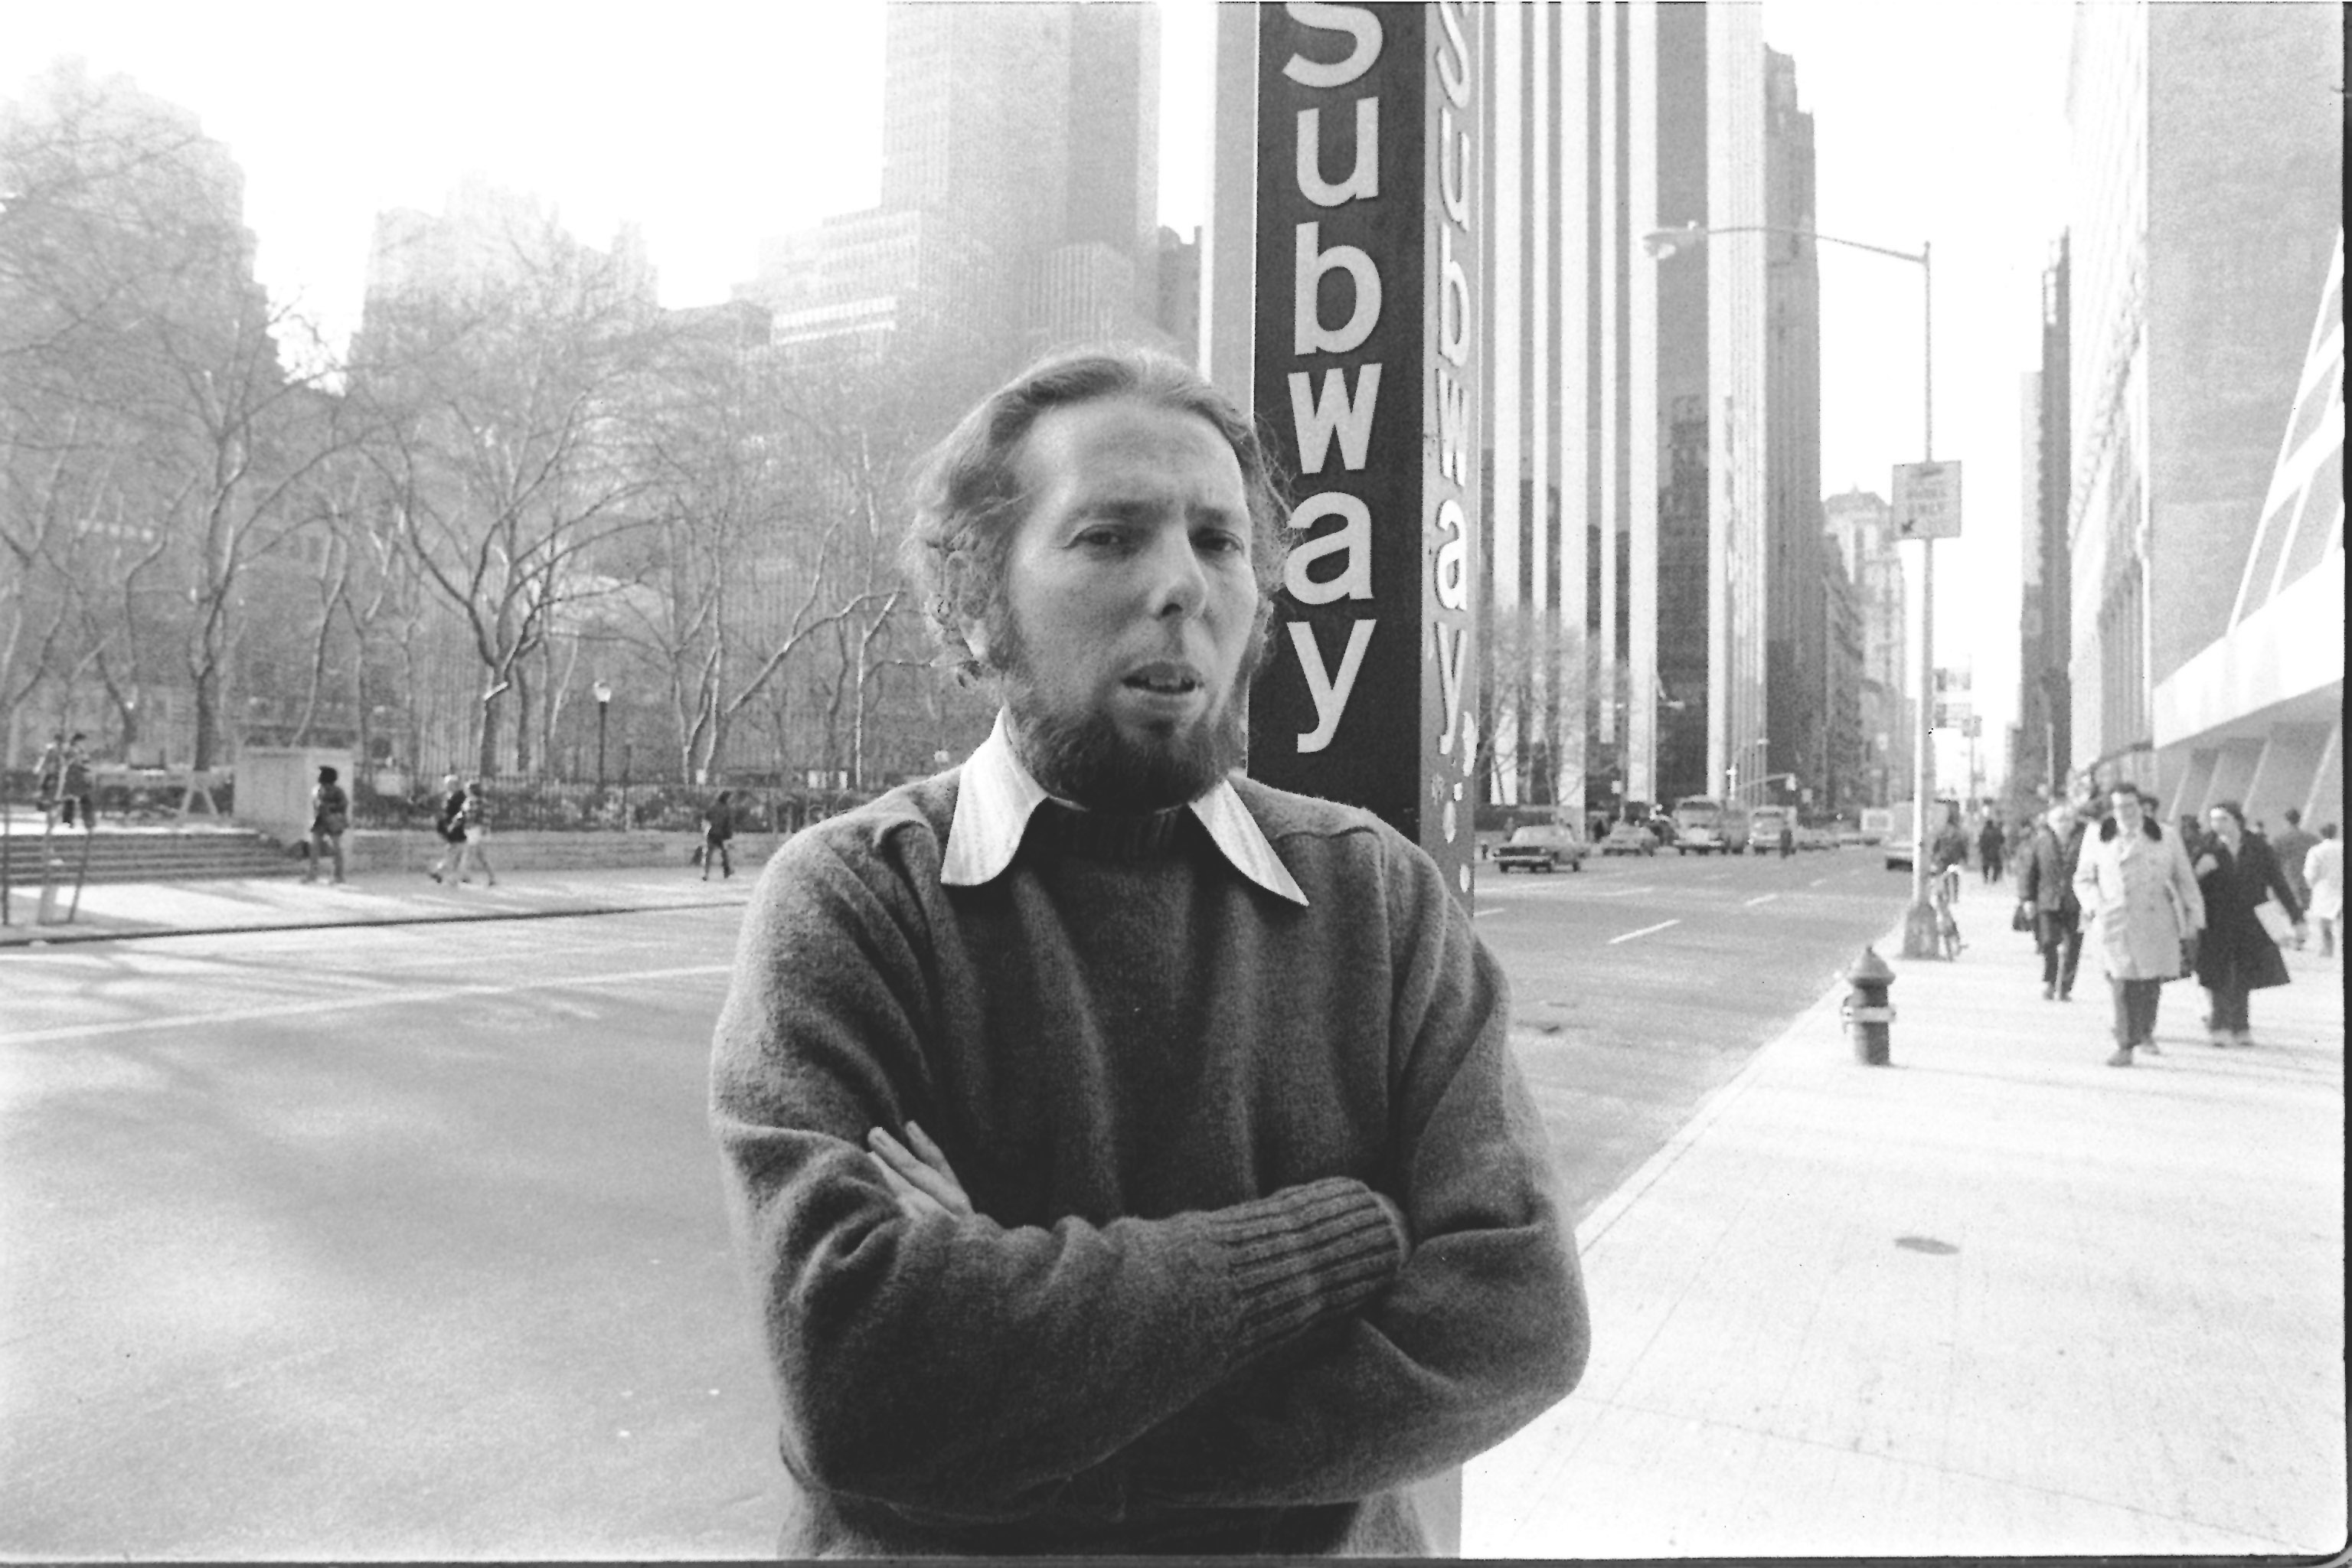
\includegraphics[keepaspectratio]{slide01_files/mediabag/KAFMHCBENYI6HMSJRGIH.jpg}}

Almost all 8 billion people on the planet are your friends of friends of
friends of friends of friends of friends.




\end{document}
